\documentclass[11pt]{article}
\usepackage[a4paper,margin=2.3cm]{geometry}
\usepackage{graphicx}
\usepackage{amsmath}
\usepackage{booktabs}
\usepackage{caption}
\usepackage[hidelinks]{hyperref}
\graphicspath{{figures/}}
\captionsetup{font=small}

\title{\vspace{-1.2cm}A distributed maturation delay in the profit--investment cycle:\\
differentiable inverse calibration and identifiability limits}
\author{Juan I. Tollo}
\date{\today}

\begin{document}
\maketitle
\vspace{-0.7cm}

\begin{abstract}
\noindent
We study the profit--investment cycle of the U.S. economy (quarterly, 1948--2026) through the
lens of overaccumulation: past investment depresses current profitability with a delay. Using
the cross-correlation function and a recession event study, we show a dominant contemporaneous
co-movement together with a negative feedback centred about one year, which builds up before
recessions---consistent with Tapia Granados (2012). Fixed-phase predator--prey oscillators
(Lotka--Volterra, FitzHugh--Nagumo) cannot reproduce this shape. We instead pose a physical
\emph{maturation-chain} model, a distributed-delay ODE, and calibrate it by a differentiable
inverse (physics-informed neural network with Fourier features). The inverse recovers the
maturation lag cleanly on synthetic data ($8.9\%$ error) and estimates $\approx\!1$ year on real
data; the lag is stable to transform choice and leave-one-crisis-out. Our central result is one
of identifiability: the \emph{centre} of the delay is robustly identified, but its
\emph{distributional width} is not, and the feedback is observationally equivalent to a linear
$\mathrm{VAR}(p\!\ge\!4)$ at the level of the second-order autocovariance.
\end{abstract}

\section{Introduction}
The Marxian tradition of overaccumulation (Astarita; Tapia Granados, 2023) holds that
capital accumulation eventually depresses the rate of profit, generating endogenous cycles and
crises. A long line of nonlinear models---starting from Goodwin's (1967) growth cycle, a
Lotka--Volterra (LV) predator--prey system, and its empirical predator--prey estimate by
Goldstein (1999)---formalises this as an antagonism between profits and a second variable. These
models impose an \emph{instantaneous} coupling with a fixed $90^\circ$ phase lag.

We ask a narrower, mechanistic question: is the feedback from investment to profits an
instantaneous antagonism, or a \emph{delayed} one whose timing reflects the maturation
(gestation) of investment? We find the latter. The empirical signature is a contemporaneous
co-movement plus a negative feedback concentrated about one year out---a shape no fixed-phase
oscillator can generate, but a distributed-delay system can. We formalise this as a physical
maturation-chain ODE and calibrate it by a differentiable inverse problem. The contribution is
descriptive and methodological: a transform-robust, leave-one-out-stable estimate of a
structural maturation lag, recovered by an inverse method where classical single-shooting fails,
together with an explicit characterisation of \emph{what cannot} be identified from these data.

\section{Data and methods}
We use quarterly U.S. corporate profits and gross private domestic investment (FRED, 1948--2026,
$n=313$). To avoid the spurious order-4 structure that the year-over-year transform injects at the
lag of interest, we work in quarter-over-quarter growth, $x_t=\Delta\log$, which we verified to
roughly halve the apparent feedback magnitude relative to YoY.

\paragraph{Descriptive.} We compute the sample cross-correlation function (CCF)
$\rho(k)=\mathrm{corr}(\text{profits}_t,\text{investment}_{t+k})$ and, around the twelve NBER
recessions, a superposed-epoch (event-study) composite aligned at the investment trough.

\paragraph{Physical model.} Investment matures through $n$ stages before depressing profits; by
the linear-chain trick this realises a Gamma-distributed delay of mean $\mu$:
\begin{equation}
\dot P = c\,I - d\,P - k\,m,\qquad
\dot I = a\,P - b\,I,\qquad
m(t)=\textstyle\sum_j w_j(\mu)\,I(t-j),
\end{equation}
with $P$ profits, $I$ investment, $m$ matured investment, and $w(\mu)$ a Gamma kernel of mean
$\mu$ (the \emph{maturation lag}).

\paragraph{Differentiable inverse.} We calibrate $(a,b,c,d,k,\mu)$ by an inverse
physics-informed neural network (PINN): a network $t\mapsto[P,I]$ trained with a data loss on the
observations and a physics-residual loss enforcing the ODE, optimising network weights and ODE
parameters jointly (loss $=\mathcal L_{\text{data}}+\lambda\mathcal L_{\text{phys}}$, $\lambda=1$;
after Raissi et al., 2019; Rackauckas et al., 2020). On long windows a plain network suffers
spectral bias and the lag collapses; \emph{Fourier-feature} inputs remove this. We validate
recovery on synthetic data with a known lag, and assess identifiability by a profile over $\mu$,
a leave-one-crisis-out analysis, and the theoretical CCF of a fitted $\mathrm{VAR}(p)$ obtained
from the discrete Lyapunov equation.

\section{Results}

\paragraph{The pattern: a delayed feedback, not an instantaneous antagonism.}
The CCF oscillates rather than decaying: a dominant contemporaneous peak ($\rho(0)\approx+0.6$)
and a negative lobe at lags $4$--$5$ quarters ($\approx-0.3$ in QoQ), returning to zero by lag~6
(Fig.~\ref{fig:ccf}). The event study (Fig.~\ref{fig:event}) shows profits turning down first and
an investment--profit gap that builds up $\sim$1--1.5 years before the trough---the
overaccumulation buildup documented by Tapia Granados (2012), here re-confirmed by an independent
method. The effective phase is near co-movement ($\sim\!10^\circ$), not the $90^\circ$ of LV/FN;
fixed-phase oscillators are accordingly refuted, as their CCF is a rigid cosine, not an isolated
pulse plus a delayed negative lobe.

\begin{figure}[t]
\centering
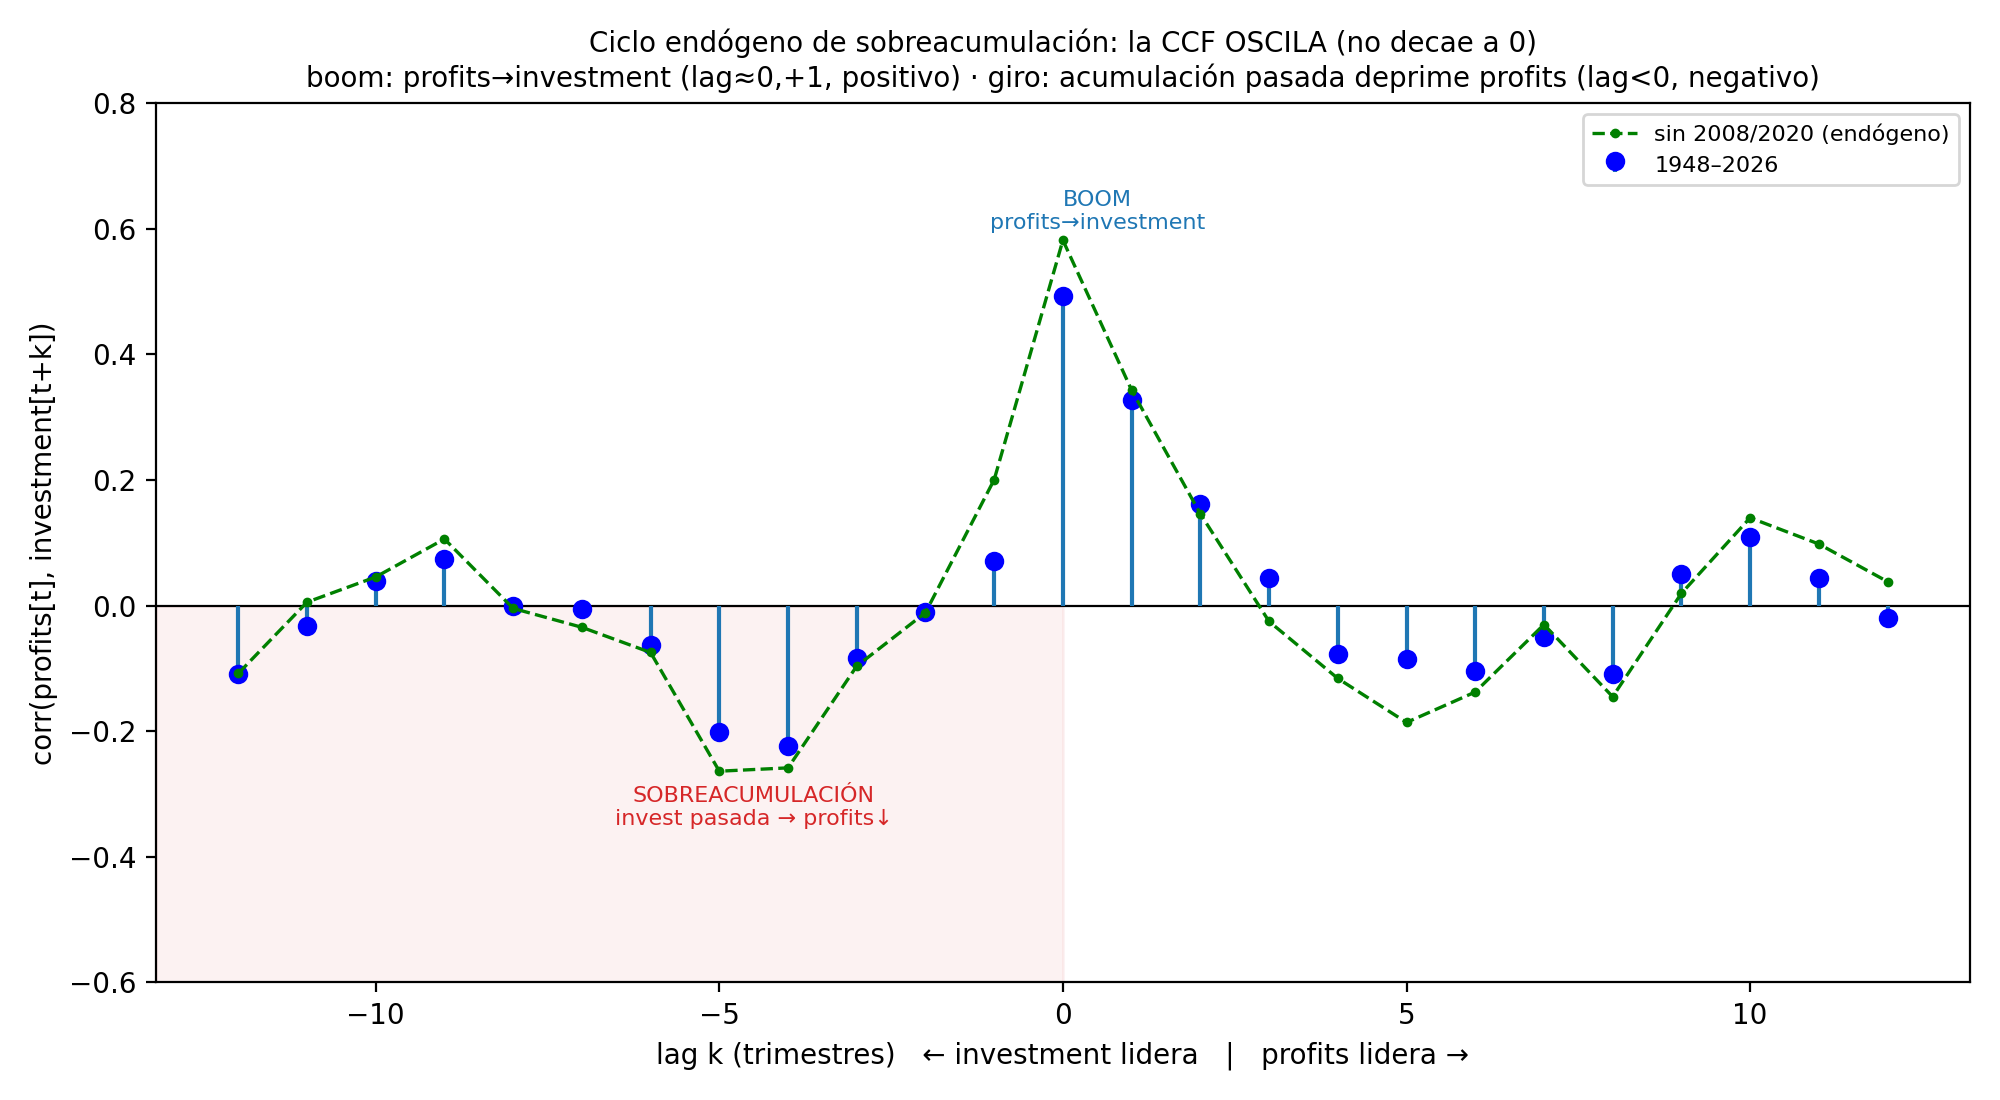
\includegraphics[width=0.74\linewidth]{p7_overaccumulation.png}
\caption{Cross-correlation profits$\leftrightarrow$investment. The function oscillates: a strong
contemporaneous co-movement and a delayed negative feedback (investment maturing $\sim$1 year
earlier depresses current profits). Robust to excluding 2008/2020.}
\label{fig:ccf}
\end{figure}

\begin{figure}[t]
\centering
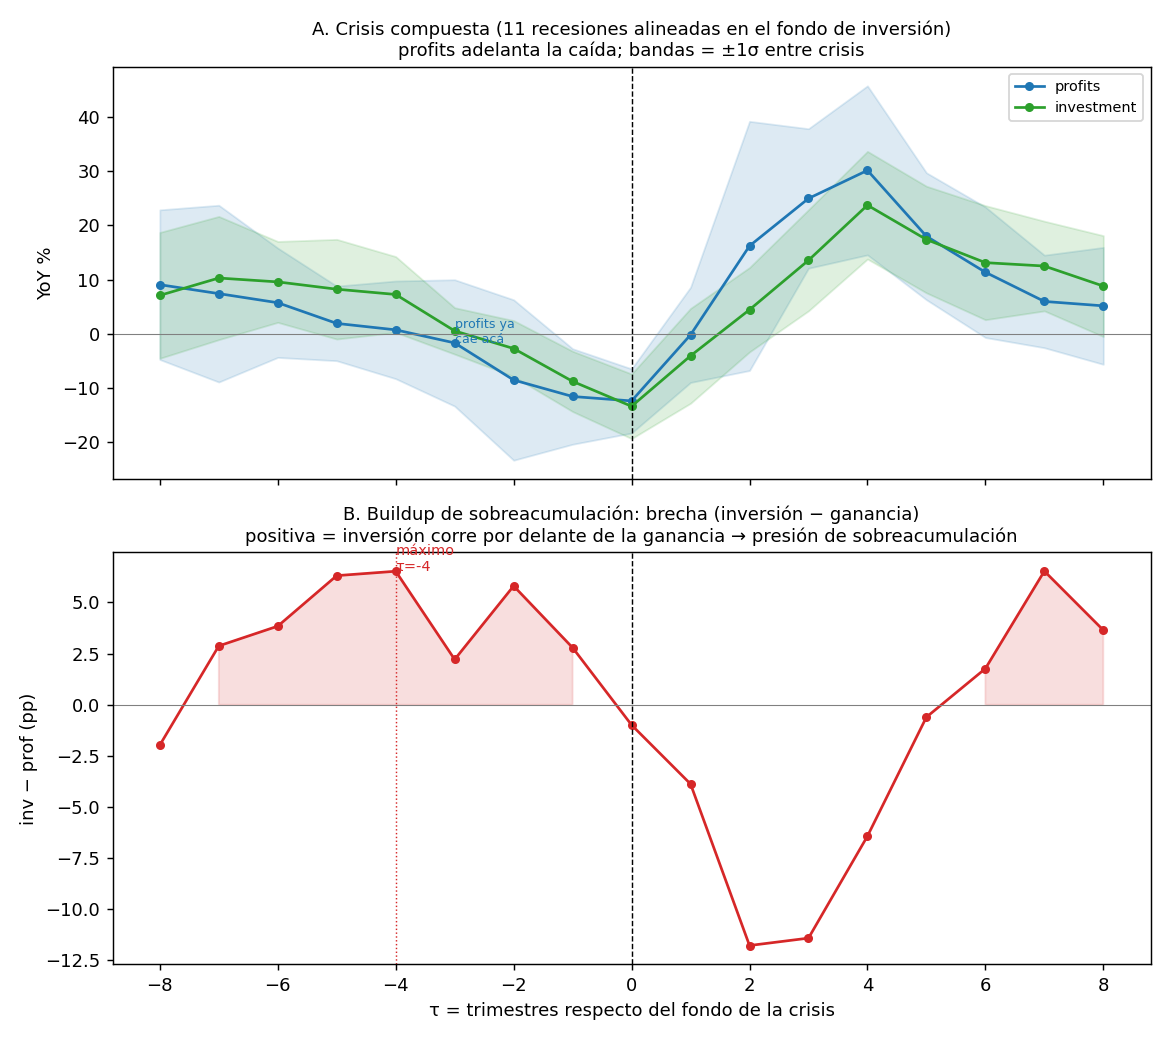
\includegraphics[width=0.74\linewidth]{p8_composite_crisis.png}
\caption{Composite of NBER recessions aligned at the investment trough. Profits lead the
downturn and the investment$-$profit gap builds up $\sim$1--1.5 years before the trough.}
\label{fig:event}
\end{figure}

\paragraph{The maturation lag is identifiable and stable.}
Five methods converge on a maturation lag of $\approx\!4$ quarters: the empirical kernel, the
distributed-lag regression, a $\mathrm{VAR}(p\!\ge\!4)$, a hierarchical pooled estimate
($\mu_{\text{pop}}\approx4.7$--$4.9$), and the differentiable inverse. The Fourier-feature inverse
PINN recovers a known synthetic lag with $8.9\%$ error ($4.0\to4.36$ quarters) and estimates
$3.90$ quarters $=0.98$ years on real data; the lag is stable across difference transforms
(QoQ, $\Delta\log$) and to leave-one-crisis-out (span $0.62$ quarter). The classical
single-shooting and the latent-state inverse fail (lag collapses or biases by $\sim\!55\%$); the
well-posed convolution form with Fourier features succeeds.

\paragraph{What cannot be identified.}
The feedback explains only $\sim\!3\%$ of the variance of profit growth (vs.\ $\sim\!35\%$ for the
contemporaneous co-movement). Consequently the \emph{width} of the delay distribution is not
identifiable (flat likelihood profile; $\mathrm{AIC}$ favours a point delay), and neither is its
variation across crises. Moreover, the negative lobe is reproduced by the theoretical CCF of a
linear $\mathrm{VAR}(p\!\ge\!4)$ from its coefficients alone (Fig.~\ref{fig:var}): the
distributed-delay kernel is \emph{observationally equivalent}, at the level of the second-order
autocovariance, to a linear stochastic system with longer memory. The maturation model is an
interpretable reparameterisation of that linear content, not a mechanism separable from it with
these data. A bifurcation analysis of the calibrated system does not yield a delay-induced Hopf
instability, so we do not claim crises to be an endogenous delayed-feedback instability.

\begin{figure}[t]
\centering
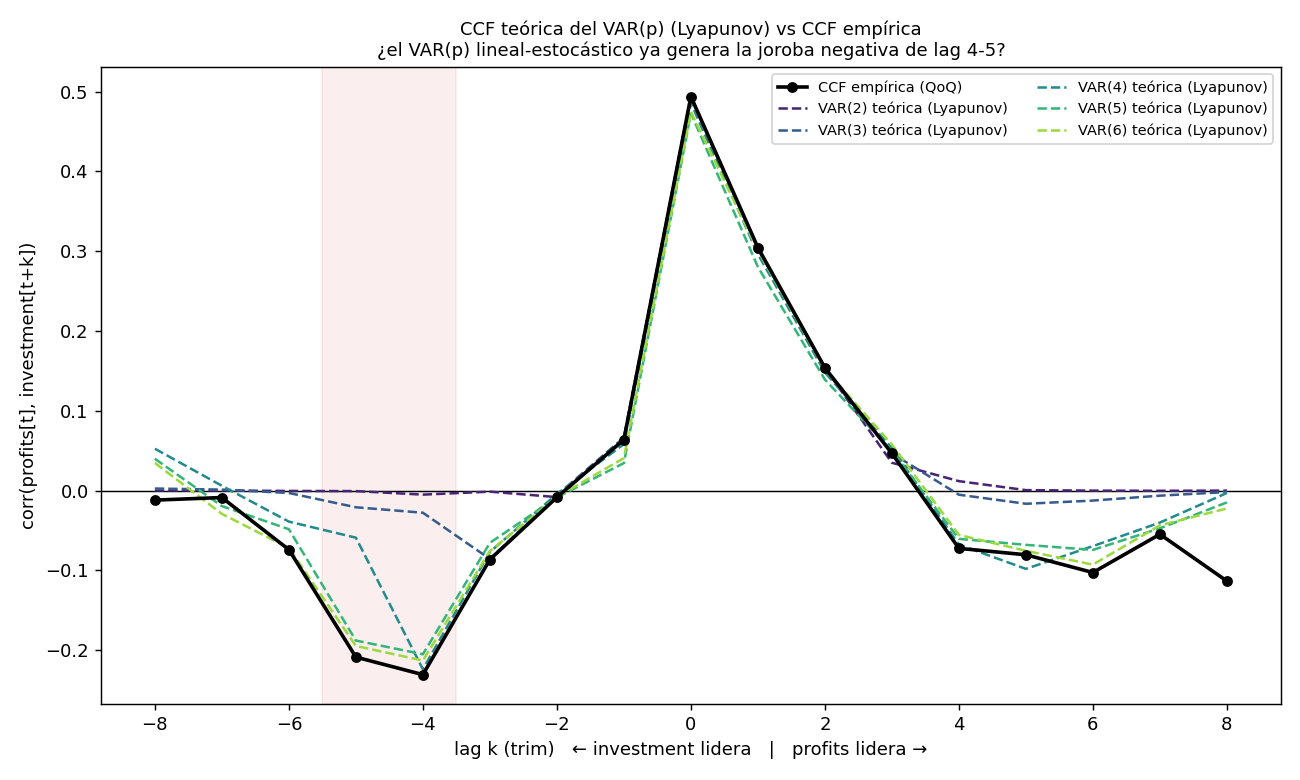
\includegraphics[width=0.62\linewidth]{p12_var_lyapunov_ccf.png}
\caption{Theoretical CCF of a fitted $\mathrm{VAR}(p)$ (Lyapunov) vs.\ the empirical CCF. For
$p\ge4$ the linear model already reproduces the negative lobe at lags 4--5 from its coefficients,
establishing observational equivalence with the distributed-delay kernel.}
\label{fig:var}
\end{figure}

\section{Discussion}
The substantive picture is consistent and honest. There \emph{is} an endogenous overaccumulation
feedback with a maturation lag of about one year, stronger near recessions, and we recover it with
a physical, differentiable model where classical inversion fails. But two limits bound the claim.
First, the economic content of the lag---its $\sim$1-year centre and pre-recession buildup---is
already in Tapia Granados (2012); our addition is the model and the inverse method, not the
phenomenon. Second, with nine usable post-war crises and a $\sim\!3\%$ signal-to-variance ratio,
the data cannot separate a genuinely \emph{distributed} (stochastic) delay from a point delay, nor
the maturation mechanism from a linear long-memory VAR. The microfoundation of a distributed delay
is the aggregation of heterogeneous investment gestation lags (Kalecki, 1935; Kydland and Prescott,
1982), so a distributed kernel is the mechanical consequence of aggregation rather than a
conjecture; but confirming its \emph{shape} requires either a multi-country panel (many more
episodes, to identify the width) or measured sectoral gestation times (to predict the macro kernel,
a test a reduced-form VAR cannot pass). These are the natural next steps.

\section{Conclusion}
The profit--investment overaccumulation feedback is well described by a distributed maturation
delay centred at $\sim$1 year, recovered by a differentiable inverse that overcomes the spectral
bias and ill-posedness of classical calibration. The robust, transferable result is the
\emph{location} of the identifiability frontier: the delay's centre is recoverable and stable,
while its width and its separation from a linear model are not---a boundary set by signal strength
and episode count, not by tuning. Pushing past it requires new data, not a reparameterisation.

\appendix

\section{Robustness and falsification battery}
\label{app:robust}
Table~\ref{tab:robust} collects the auxiliary tests. Two points are worth stressing. First, the
\emph{location} of the lag ($\approx\!5$ quarters) is stable within the difference family
(QoQ, $\Delta\log$) and to leave-one-crisis-out (Fig.~\ref{fig:stab}, left; pooled
$\mu\approx4.7$, span $0.62$), although per-crisis confidence intervals are wide because the
feedback is weak and identification emerges only by pooling. Second, the negative lobe is
\emph{not} a clean crisis-specific signature: a kernel placebo over non-crisis windows finds it
roughly as often off-crisis, and a $\mathrm{VAR}(p\!\ge\!4)$ reproduces it from its coefficients
(main text, Fig.~3). The year-over-year transform both inflates the magnitude $\sim2\times$ and
shifts the apparent lag (to $\sim2$ quarters), and two-sided cycle filters (HP, band-pass)
collapse it to a contemporaneous term---so we report QoQ throughout (Fig.~\ref{fig:stab}, right).

\begin{table}[h]\centering\small
\begin{tabular}{@{}lll@{}}
\toprule
Test & Question & Result \\
\midrule
Transform robustness & lag location robust to transform? & $\mu^\star\!\approx\!5$q (QoQ/$\Delta\log$); YoY$\to$2q; filters$\to$1q \\
Lag stability / LOO & lag stable across crises? & pooled $\mu\!\approx\!4.7$q; LOO span $0.62$q; all in CI \\
Hierarchical pooling & population lag \& spread & $\mu_{\text{pop}}\!\approx\!4.9$q $[4.4,5.5]$; spread contested \\
Kernel placebo & is the 4--5q lobe crisis-specific? & ubiquitous (appears off-crisis too) \\
VAR$(p)$ Lyapunov & does a linear VAR reproduce it? & yes for $p\!\ge\!4$ $\Rightarrow$ obs.\ equivalence \\
Pooled-dynamics placebo & is shared crisis dynamics special? & preliminary: ratios $\approx$ crisis $\Rightarrow$ not special \\
\bottomrule
\end{tabular}
\caption{Auxiliary robustness and falsification tests. The lag's centre is robust; its
crisis-specificity and its separation from a linear model are not.}
\label{tab:robust}
\end{table}

\begin{figure}[h]
\centering
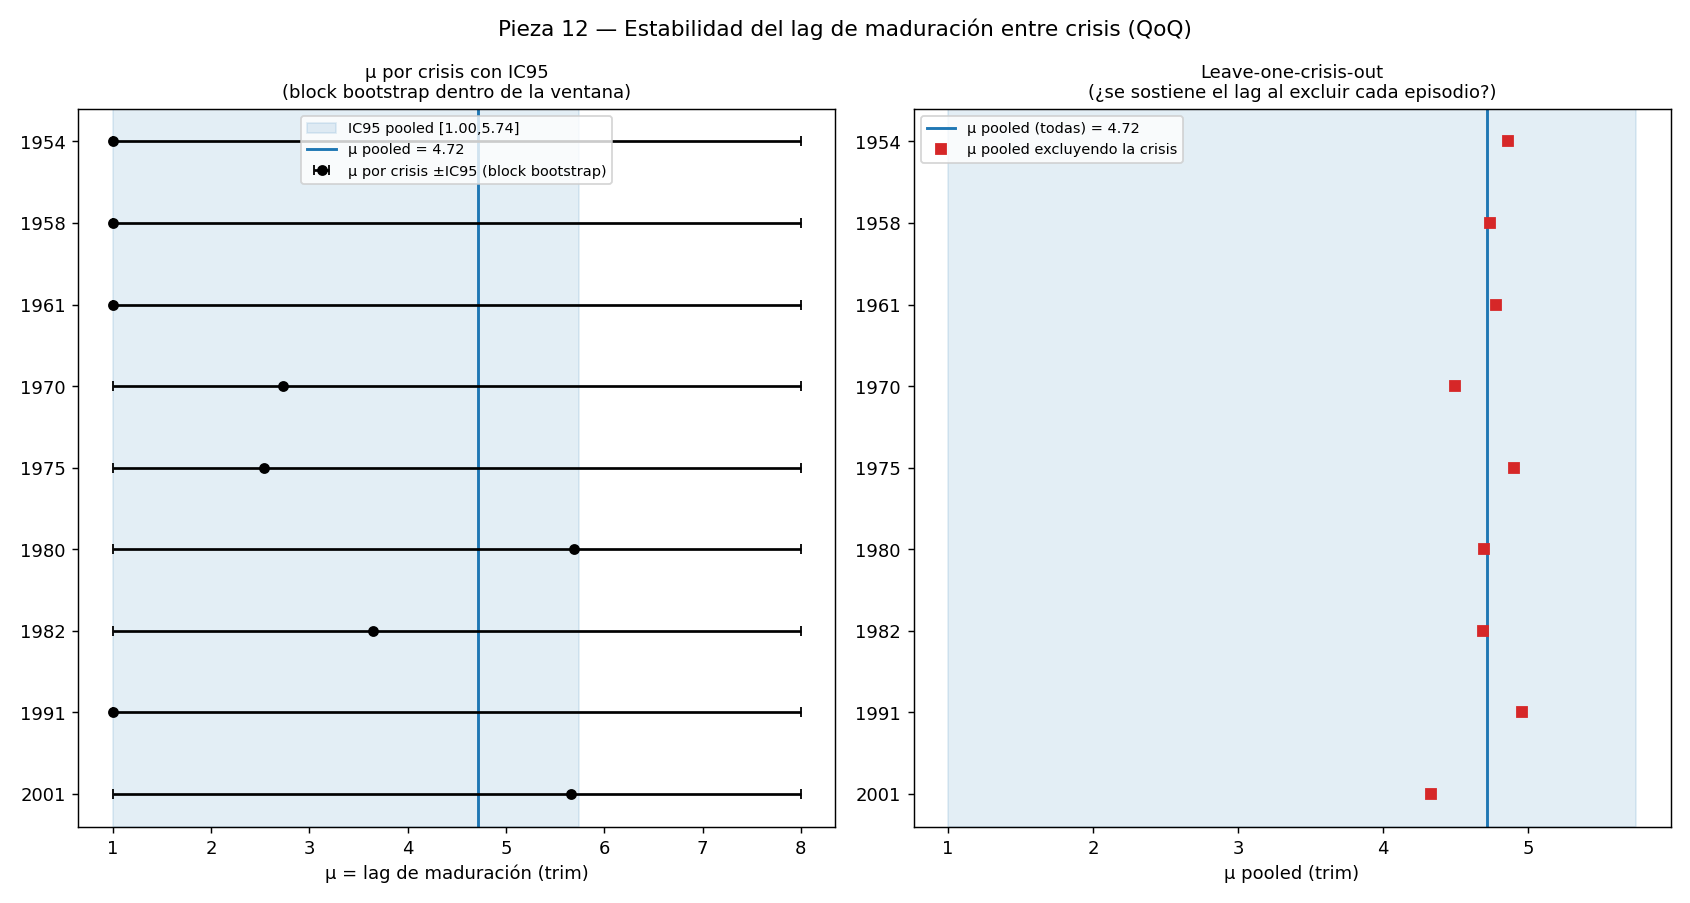
\includegraphics[width=0.49\linewidth]{p12_lag_stability.png}\hfill
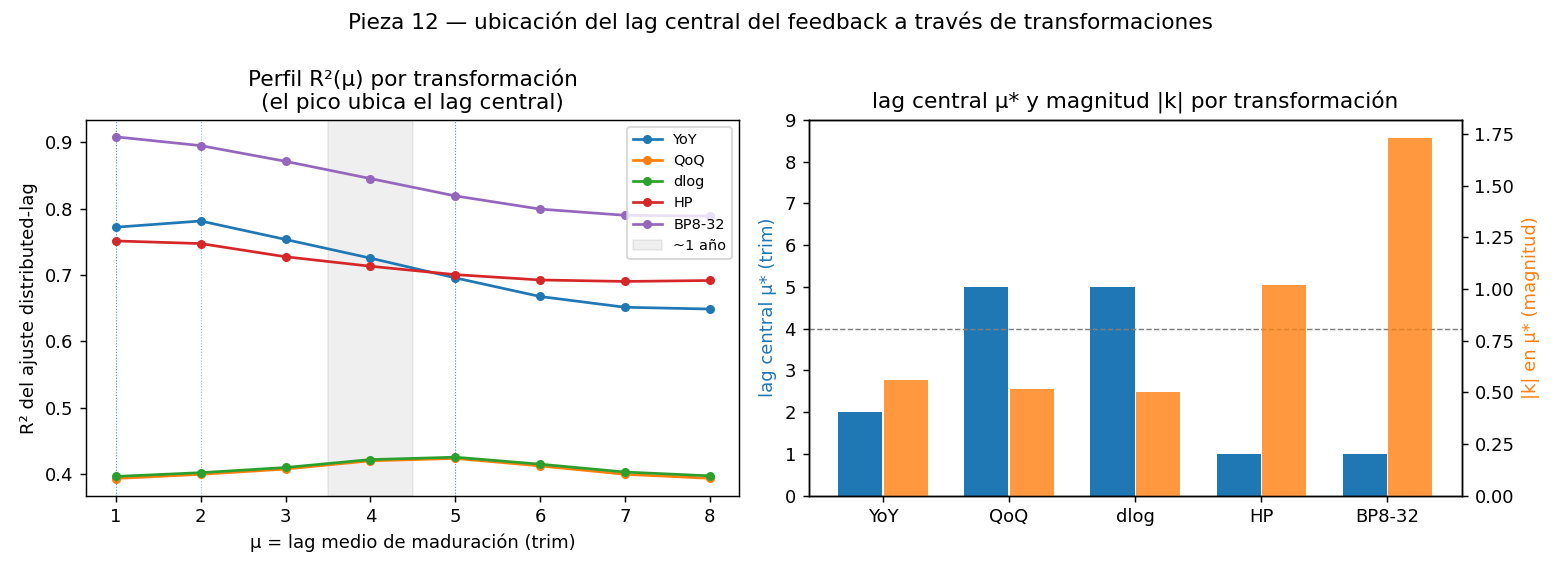
\includegraphics[width=0.49\linewidth]{p12_transform_robustness.png}
\caption{Left: per-crisis maturation lag with leave-one-crisis-out (the pooled lag does not
depend on any single episode). Right: estimated lag location under different transforms; stable
within the difference family, shifted by YoY and by two-sided cycle filters.}
\label{fig:stab}
\end{figure}

\section{Inverse-PINN variants and a stability check}
\label{app:pinn}
The maturation lag is recoverable by the differentiable inverse only when the surrogate network
can represent the series and the parameters are well-posed. Table~\ref{tab:pinn} compares four
variants on synthetic data (true lag $4$ quarters) and on the real window. A plain network on the
long window suffers spectral bias and the lag collapses; per-crisis pooling fixes the fit
($\bar R^2\!=\!0.86$) but not the lag; only \emph{Fourier-feature} inputs recover the lag cleanly
($8.9\%$ synthetic error, $0.98$ years real). Finally, a bifurcation analysis of the calibrated
system (Fig.~\ref{fig:bif}) finds \emph{no} delay-induced Hopf instability: the system's
instability comes from low damping, not from the lag, and the structural fit even disagrees with
the distributed-lag estimate on $\mu$. We therefore do not advance an ``endogenous
delayed-feedback instability'' claim---it would require the stronger identification that a panel
or micro gestation data could provide.

\begin{table}[h]\centering\small
\begin{tabular}{@{}llll@{}}
\toprule
Variant & Synthetic (true $4$q) & Real lag & Verdict \\
\midrule
Single-shooting / convolution & $1.86$q ($54\%$ err) & collapses to $0.23$q, non-physical & fails \\
Per-crisis pooled & $1.64$q ($59\%$ err) & $0.84$q ($\bar R^2\!=\!0.86$) & fits, lag collapses \\
Profile-likelihood in $\mu$ & --- & inconclusive & unstable \\
\textbf{Fourier features} & $\mathbf{4.36}$\textbf{q} $\mathbf{(8.9\%)}$ & $\mathbf{3.90}$\textbf{q}$=\mathbf{0.98}$\textbf{yr} ($R^2\!=\!1$) & \textbf{recovers} \\
\bottomrule
\end{tabular}
\caption{Inverse-PINN variants. Only Fourier-feature inputs both fit the series and recover the
maturation lag; the others fail through spectral bias or the $k$--$\mu$ trade-off.}
\label{tab:pinn}
\end{table}

\begin{figure}[h]
\centering
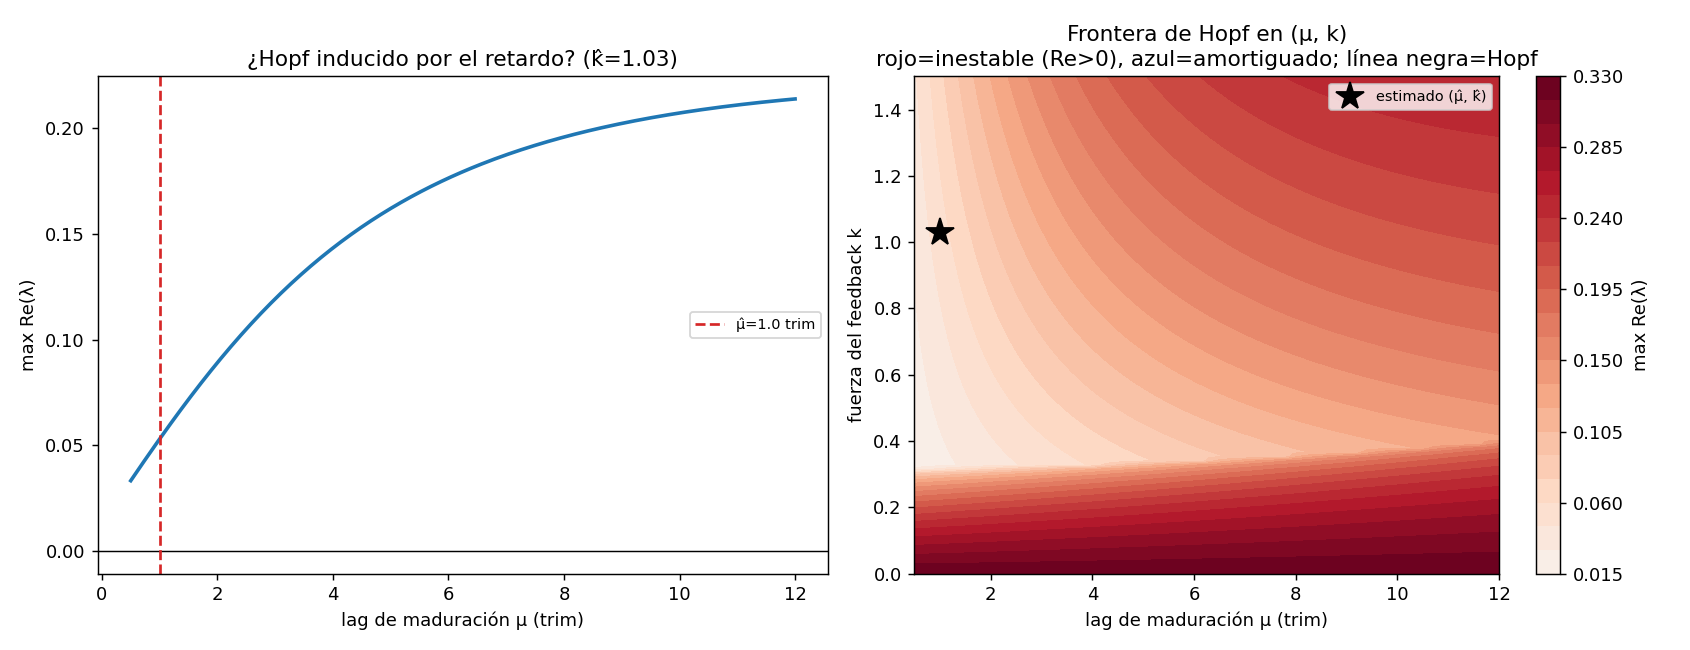
\includegraphics[width=0.84\linewidth]{p13_bifurcation.png}
\caption{Stability of the calibrated maturation system. Left: maximum $\mathrm{Re}(\lambda)$ vs
the lag $\mu$; no zero-crossing, i.e.\ no delay-induced Hopf. Right: the Hopf boundary in
$(\mu,k)$ with the estimate marked. The mechanistic ``instability'' reading is not supported by
these data.}
\label{fig:bif}
\end{figure}

\begin{thebibliography}{9}\small
\bibitem{almon} Almon, S. (1965). The distributed lag between capital appropriations and
expenditures. \emph{Econometrica} 33(1), 178--196.
\bibitem{goldstein} Goldstein, J.P. (1999). Predator--prey model estimates of the cyclical profit
squeeze. \emph{Metroeconomica} 50(2), 139--173.
\bibitem{goodwin} Goodwin, R.M. (1967). A growth cycle. In \emph{Socialism, Capitalism and
Economic Growth}. Cambridge University Press.
\bibitem{kalecki} Kalecki, M. (1935). A macrodynamic theory of business cycles.
\emph{Econometrica} 3(3), 327--344.
\bibitem{kp} Kydland, F.E., Prescott, E.C. (1982). Time to build and aggregate fluctuations.
\emph{Econometrica} 50(6), 1345--1370.
\bibitem{raissi} Raissi, M., Perdikaris, P., Karniadakis, G.E. (2019). Physics-informed neural
networks. \emph{Journal of Computational Physics} 378, 686--707.
\bibitem{rackauckas} Rackauckas, C., et al. (2020). Universal differential equations for
scientific machine learning. \emph{arXiv:2001.04385}.
\bibitem{ramsay} Ramsay, J., Hooker, G. (2017). \emph{Dynamic Data Analysis}. Springer.
\bibitem{tapia} Tapia Granados, J.A. (2012). Statistical evidence of falling profits as cause of
recession. \emph{Review of Radical Political Economics} 44(4), 484--493.
\end{thebibliography}

\end{document}
